\documentclass[12pt]{article}
\usepackage[utf8]{inputenc}
\usepackage[
top=2cm,
bottom=2cm,
left=3cm,
right=2cm,
headheight=17pt, % as per the warning by fancyhdr
includehead,includefoot,
heightrounded, % to avoid spurious underfull messages
]{geometry} 
\geometry{a4paper}
\usepackage[ngerman]{babel}
\usepackage{listings}
\usepackage{fancyhdr}
\usepackage{siunitx}
\usepackage{graphicx}
\usepackage{caption}
\usepackage[table]{xcolor}
\fancyhf{}
\fancyhead[CO,CE]{Parallel Computer Architecture: Exercise 2}
\fancyfoot[C]{Group 04}
\fancyfoot[RO, LE] {\thepage}
\renewcommand{\headrulewidth}{0.4pt}
\renewcommand{\footrulewidth}{0.4pt}
\pagestyle{fancy}

% Assembler
\lstdefinelanguage
{Assembler} % based on the "x86masm" dialect
% with these extra keywords:
{morekeywords={call, mov}} % etc.



\begin{document}
	\begin{titlepage}
		\centering

		{\scshape\LARGE Universität Heidelberg \par}
		\vspace{1cm}
		{\scshape\Large Parallel Computer Architecture \par}
		\vspace{1.5cm}
		{\huge\bfseries Exercise 2\par}
		\vspace{2cm}
		{\Large\itshape Barley, Daniel\\Barth, Alexander\\Nisblé, Patrick\par}
		\vfill
		
		
		% Bottom of the page
		{\large Due date: 2019-11-08, 14:00\\Group 04\par}
	\end{titlepage}
\setcounter{section}{2}
\subsection{Matrix-Vektor-Multiplikation}

\setcounter{subsubsection}{1}
\subsubsection{Experimente und Evaluation}

\noindent \textbf{a.}

\begin{table}[ht]
	\centering
	\caption[Messwerte]{Messwerte}
	\begin{tabular}{c|l|l|l}
		\hline
		\cellcolor{gray!40}\textbf{M $\times$ N} & \multicolumn{1}{c}{\cellcolor{gray!40}\textbf{$t_{row}$(\si{\second})}} & \multicolumn{1}{c}{\cellcolor{gray!40}\textbf{$t_{col}$(\si{\second})}} & \multicolumn{1}{c}{\cellcolor{gray!40}\textbf{Ratio}}\\
		\hline\hline
		10 $\times$ 10 & \num{8.545e-6} & \num{1.1626e5} & 0.73499054\\\hline
		100 $\times$ 100 & 0.000254222 & 0.000722013 & 0.35210169\\\hline
		500 $\times$ 500 & 0.005989163 & 0.016997692 & 0.35235154\\\hline
		1000 $\times$ 1000 & 0.023987485 & 0.069154029 & 0.34687039\\\hline
		5000 $\times$ 5000 & 0.60724551 & 1.7547349 & 0.34606111\\\hline
		10000 $\times$ 10000 & 2.4371004 & 7.2018543 & 0.33839902\\\hline
	\end{tabular}
	\label{tab:values}
\end{table}

\noindent \textbf{b.}

Beim spaltenweisen Zugriff wird nur ein Teilsummand von $y_i$ berechnet.


\noindent \textbf{c.}

\begin{figure}[ht]
	\centering
	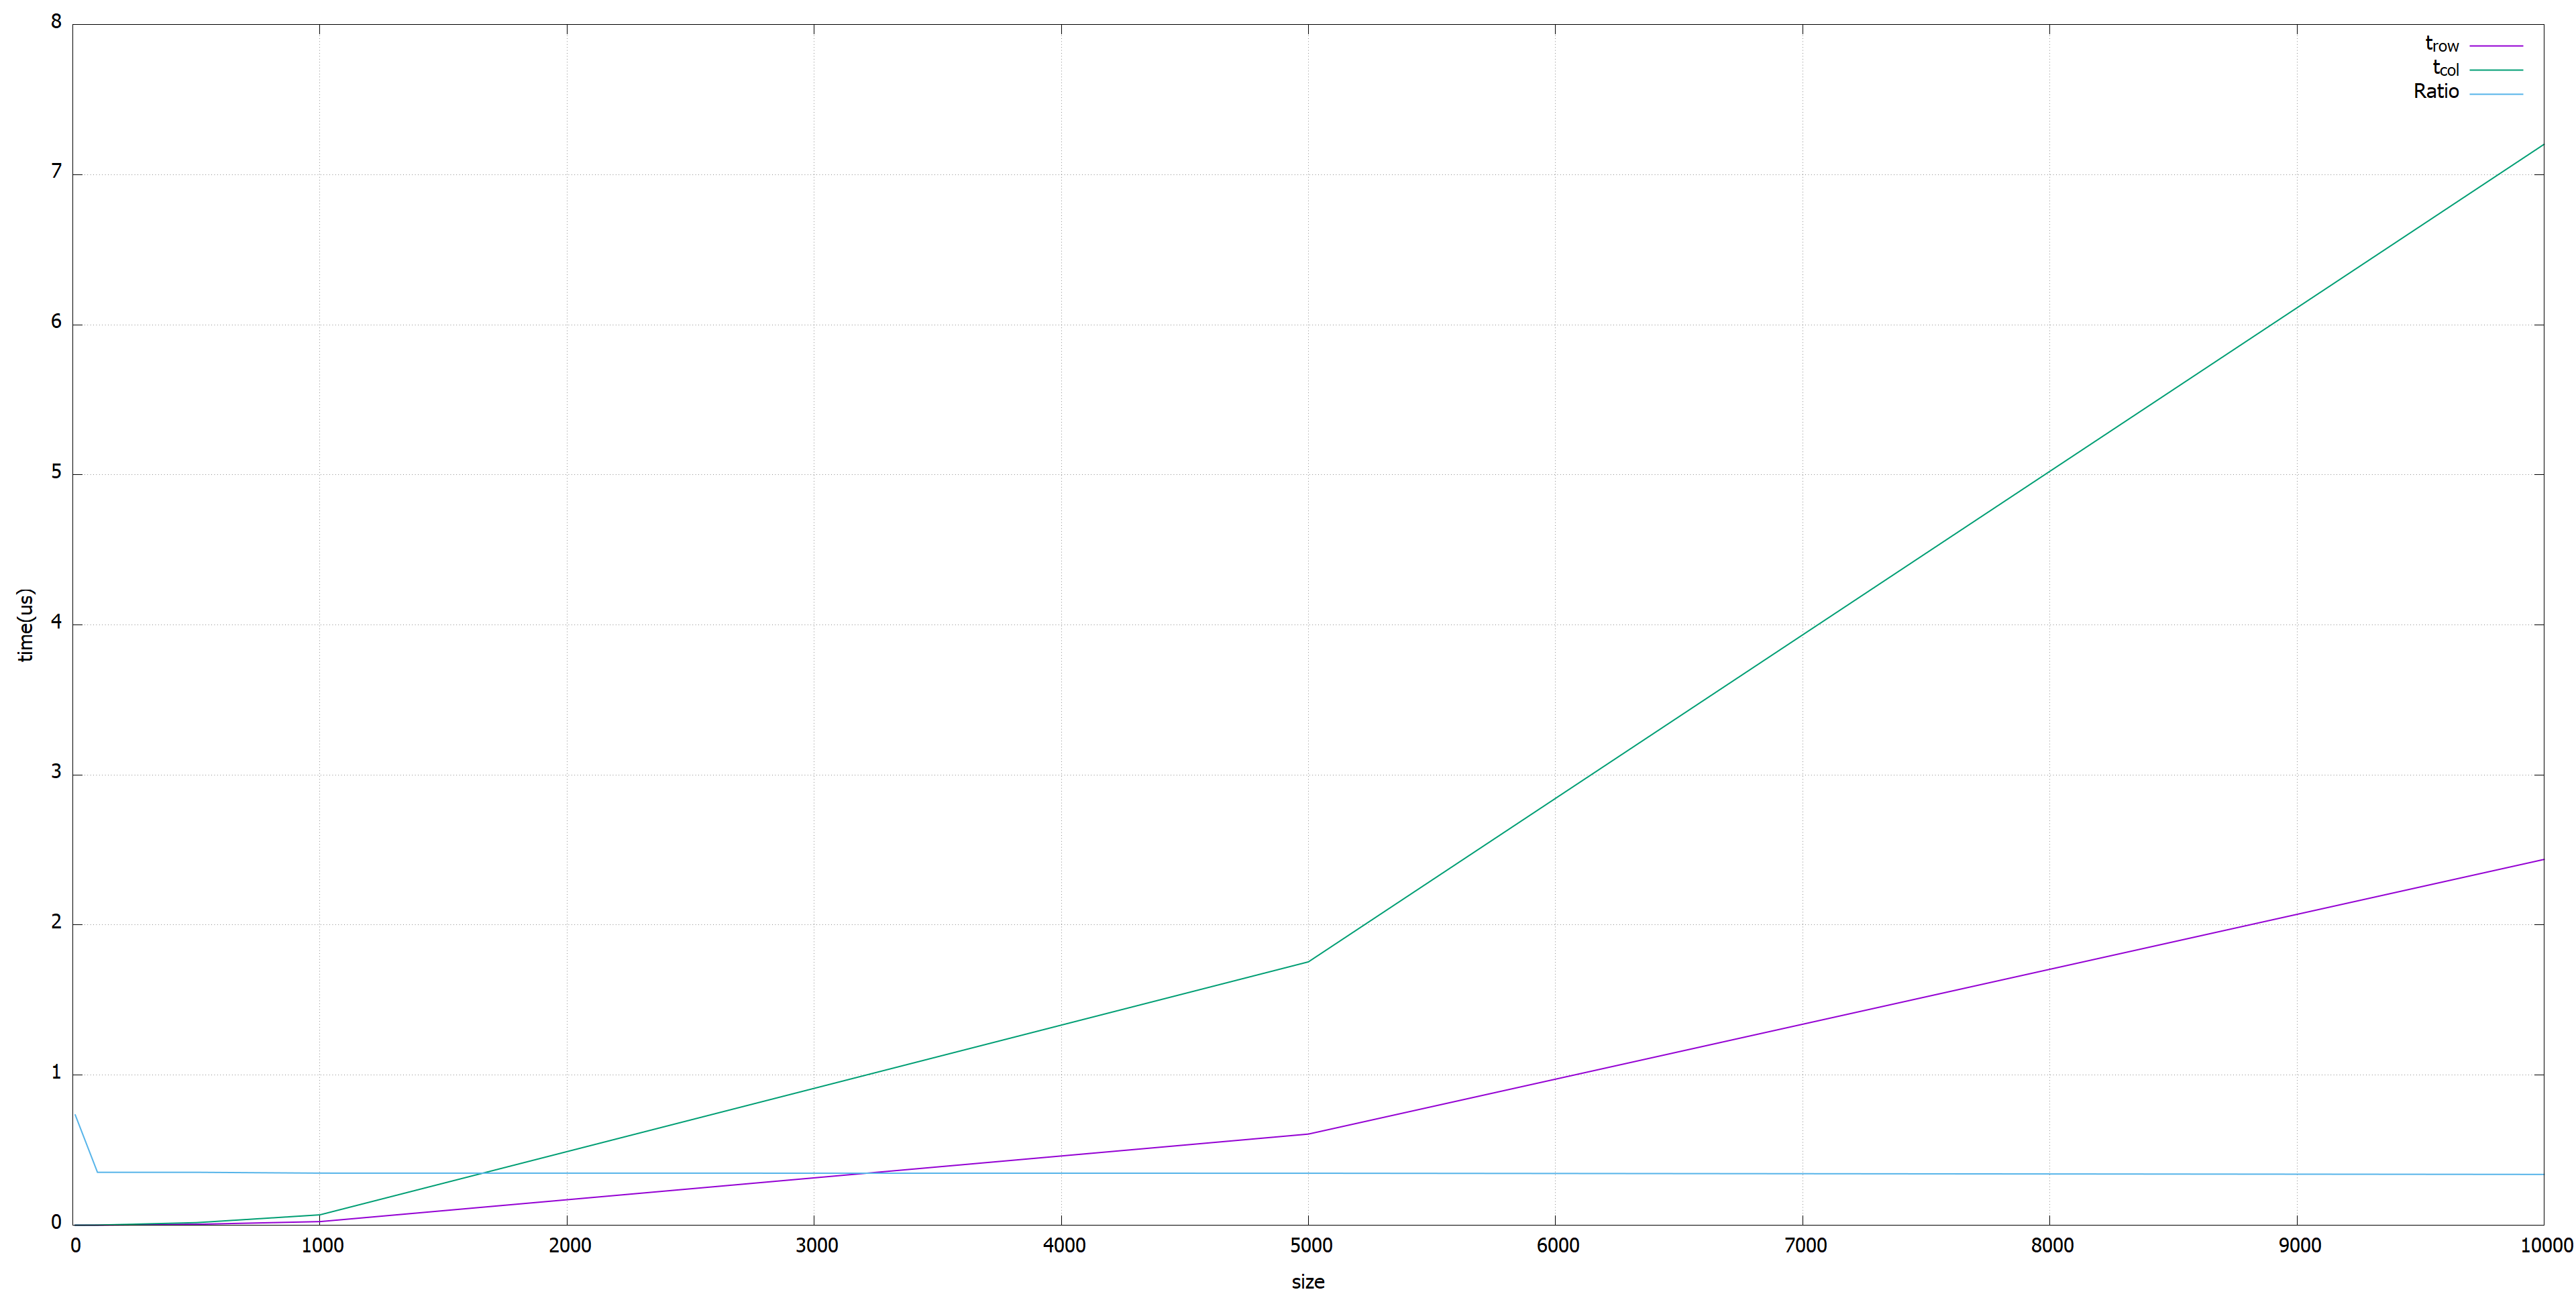
\includegraphics[width=0.9\linewidth]{../plot}
	\caption[Messwerte]{Messwerte}
	\label{fig:plot}
\end{figure}

\end{document}